%%____________________________________________________________________________||
\section{Systematic uncertainties}
\label{sec:systematics}


Two types of systematic uncertainty are considered separately. Normalisation uncertainties 
and uncertainties associated with the \mht templates for each individual (\njet,~\nb,~\scalht).



\subsection{Systematic uncertainties in the transfer factors}

To derive the normalisation uncertainties for each (\njet,~\nb,~\scalht) bins we use use of ensembles of ``closure tests''.

\label{sec:bkgdnorm-syst}

The transfer factors are obtained from simulations and an appropriate systematic uncertainty has to be assigned
for each transfer factor to account for limitations in the simulation modelling of event kinematics
 and instrumental effects. 

The sensitivity of the transfer factors to systematic sources are determined by performing a set of closure test.
 A large ensemble (\ie hundreds) of closure tests are performed between a number of control (sub-)samples.

Consitency of the set of predictions if then studied and expressed as the ratio $(\nobs - \npre)/\npre$, while considering only
the statistical uncertainties on \npre and \nobs. 

If statistically significant biases are observed, further studies are performed to understand and correct for
these biases.


The closure tests rely on the \mj, \mmj, and \gj control samples. Specific closure tests probe different sources of uncertainties. 
For example the \mj $\rightarrow$ $\gamma$ + jets tests deal with the consistency
of the prediction of \wej with $\gamma$ + jets. The $\mj \rightarrow \mmj$ tests also addresses the modelling of
vector boson production and the $\mmj \rightarrow \gj$ tests deal with the consistency between the \zee + jets and $\gamma$ + jets samples, which
is a further check on the validity of using the \gj process to predict the \znunu\, + jets process. The muon trigger and reconstruction
efficiencies are also indirectly probed, given that different numbers of muons are required in each of the two sub-samples.
%However, dedicated data-driven methods are used to measure the muon
%trigger and reconstruction efficiencies, with values taken from the
%muon POG.

To test the prediction of \znunu + jets processes with the $W$-enriched \mj control sample
the $\mu^{+}\rightarrow\mu^{-}$ closure test is used. The $0$ b-tag $\rightarrow1$ b-tag and $1$ b-tag $\rightarrow2$ b-tag
tests probe the sensitivity of the transfer factors to the relative admixture of events from the $W$ + jets and \ttbar processes by
varying the number of b-tagged jets within the \mj sample. 

These tests are conservative, as the admixture changes little between the \mj sample and the signal region 
(as there is no extrapolation in \nb), whereas the closure tests use sub-samples with different \nb bins and
therefore different admixtures of $W$ + jets and \ttbar events. \eg, the former uses a $W$-enriched sub-sample (selected by requiring zero
b-jets) to predict yields in a \ttbar-enriched sub-sample (selected by requiring one b-jet).

The $\njet=2\rightarrow\njet=3$ and $\njet=4\rightarrow\njet\geq5$ tests are an agressive test of the simulation modelling of jet
multiplicities in the \mj, \mmj and \gj samples, which is checked due to the exclusive binning in jet multiplicity. The different \njet
requirements also lead to different admixture of W + jets and \ttbar in the case of the \mj sample.

The TT$\rightarrow$TL closure tests are designed to test the effects of the extrapolation in the
 lepton definition used for the veto in the signal region (see Sec.~\ref{sec:vetoes}) and the selection in the
muon control regions. 

Finally, closure tests that probe the modelling of the \alphat and \bdphi extrapolations in the analysis are also performed. 
In both cases, the test checks if events with genuine \met found in the core of the variable distribution below some 
threshold value can be used to predict the events in the tail (above the same threshold value). 


The systematic uncertainties associated with the transfer factors are determined from ensembles of closure
tests. The statistical precision of these tests is taken into account as it limits the knowledge whether closure is actually achieved or otherwise. 
Ensembles comprising several tests are considered in bins of (\njet,\scalht) to derive a systematic uncertainty for that bin. These systematic uncertainties are then considered a ``normalisation'' uncertainty for the background predictions. These are treated fully fully uncorrelated between the (\njet,~\nb)
categories and \scalht bins. 

%Example of a closure test is given in Fig.~\ref{fig:ZinvclosureDataSymlt400}. The remaining ones can be found in~\cite{alphaTnote}.
All closure tests can be found in ~\cite{alphaTnote}.


In some kinematically restricted bins, such as those with a high jet multiplicity and low value of \scalht, the
limited statistics leads to large systematic errors. These bins are not used in the analysis. 
In the bins populated with a reasonable number of events, the systematic errors determined from the closure tests vary from $10$ to
$40\%$.


\section{Systematic uncertainties in the \mht dimension}

An additional systematic to be considered is the shape of the \mht distribution in each signal region category. 
A data driven approach is utilised in which the shape of data driven control regions is compared to the \mht shape from simulations.
For each Data/MC ratio of the shape in each signal category bin the first order polynomial is fitted. The result of this fit - a linear bias - 
is then used as systematic uncertainty and propagated through the likelihood model.
This approach has been validated in 8 TeV data. 


%By anchoring the scale using binning in the \scalht dimension the remaining
%bias should be negligible. In Figs.~\ref{fig:linearFits0bLe3} and \ref{fig:linearFits0bGe4} 
%example fits of an orthogonal linear function to the data/MC ratio 
%are shown for the three control regions. Comparing to the inclusive distribution 
%the linear component can be seen to be compatible with the null hypothesis, 
%i.e. no bias. In order to formalise this assertion 
%the pull of the linear component from zero is calculated.
%This pull distribution is shown for each of the three control regions in
%in Fig.~\ref{fig:pulls} and can be seen in each case to have mean and sigma
%consistent with zero and one respectively. This confirms that the linear component 
%is compatible with zero ($p_1 = 0$), i.e. no significant bias is observed, 
%and the uncertainty on the parameter is correctly estimated by the fit.
%Fig.~\ref{fig:frenchFlagPulls} shows the distribution of the pulls 
%in category and \scalht bins. Those anchored by \scalht are consistent
%with zero (including inclusive jet categories) while the fits inclusive in \scalht
%show very large pulls. This shows, as expected, the \scalht anchoring
%is critical for removing bias in the \mht dimension. The linear fits to the
%data/MC ratio additionally show a p-value following 
%a uniform distribution between 0 and 1 as shown in Fig.~\ref{fig:pValues}.


Each background in the signal region (\ttbar/W  and \zInv~) is predicted  using several control regions. 
In order to determine the uncertainty in the \mht dimension a combined linear fit is made over all relevant control regions
of the linear function. A requirement of at least 10 events and a non-trivial number of degrees of freedom
 is made to ensure a reasonable fit. Where this requirement is not satisfied the \mht distribution is not used in the signal region.
An \mht requirement of 130 \GeV is made to ensure a similar phase space to the signal region.
The uncertainty on the linear parameter from the fit is then used to define the up and down one sigma variations of the nominal template.
As a conservative estimate, the best fit value of the parameter is added in quadrature to its uncertainty in order to derive the overall variation.

This method has been validated in 8 TeV data and an additional validation is carried out by comparing expected and observed uncertainties
on the linear parameter defining the template variations.



\subsection{Expected systematic uncertainties for the 13 \texorpdfstring{\TeV} analysis}
Using the method described expected relative uncertainties per \GeV from 13 \TeV MC for both \ttbar/$W$  and \zInv~ using all relevant control regions are
shown in Fig.~\ref{fig:expected13} for 3\ifb. An example of the overall uncertainties on the \mht templates is shown
in Figure~\ref{fig:exampleTemplate13}. The alternative templates derived with this method are folded into the 
likelihood described in Section~\ref{sec:likelihood} to account for systematic uncertainties in the \mht dimension.


%\begin{figure}[h!]
%  \centering
%  \subfigure[\label{fig:ttw13} \ttbar/W]{
%    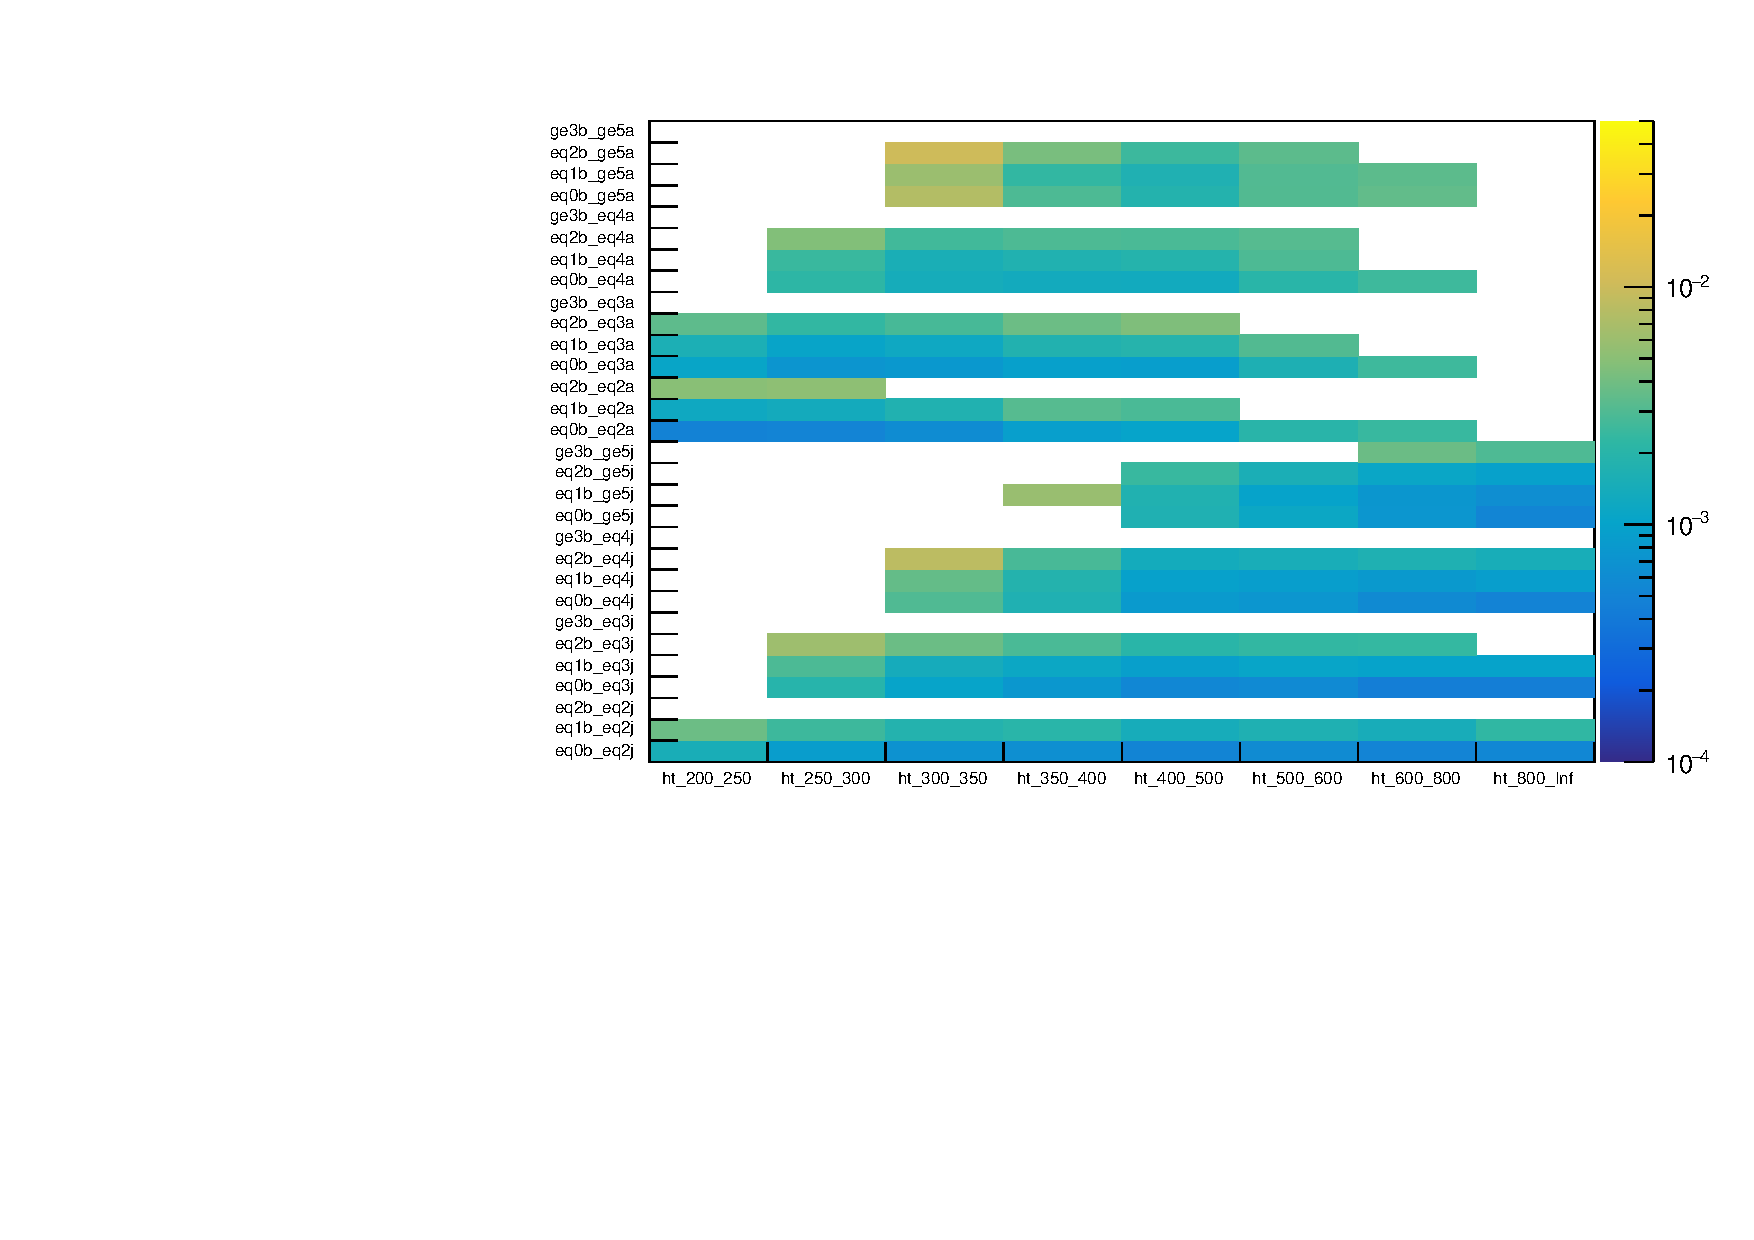
\includegraphics[width=0.5\textwidth]{figures/template13TeV//3fb/frenchFlagErrComplete_Linear2DShiftMean_p1_Ttw.pdf}
%  }~~
%  \subfigure[\label{fig:zinv13} \zInv~]{
%    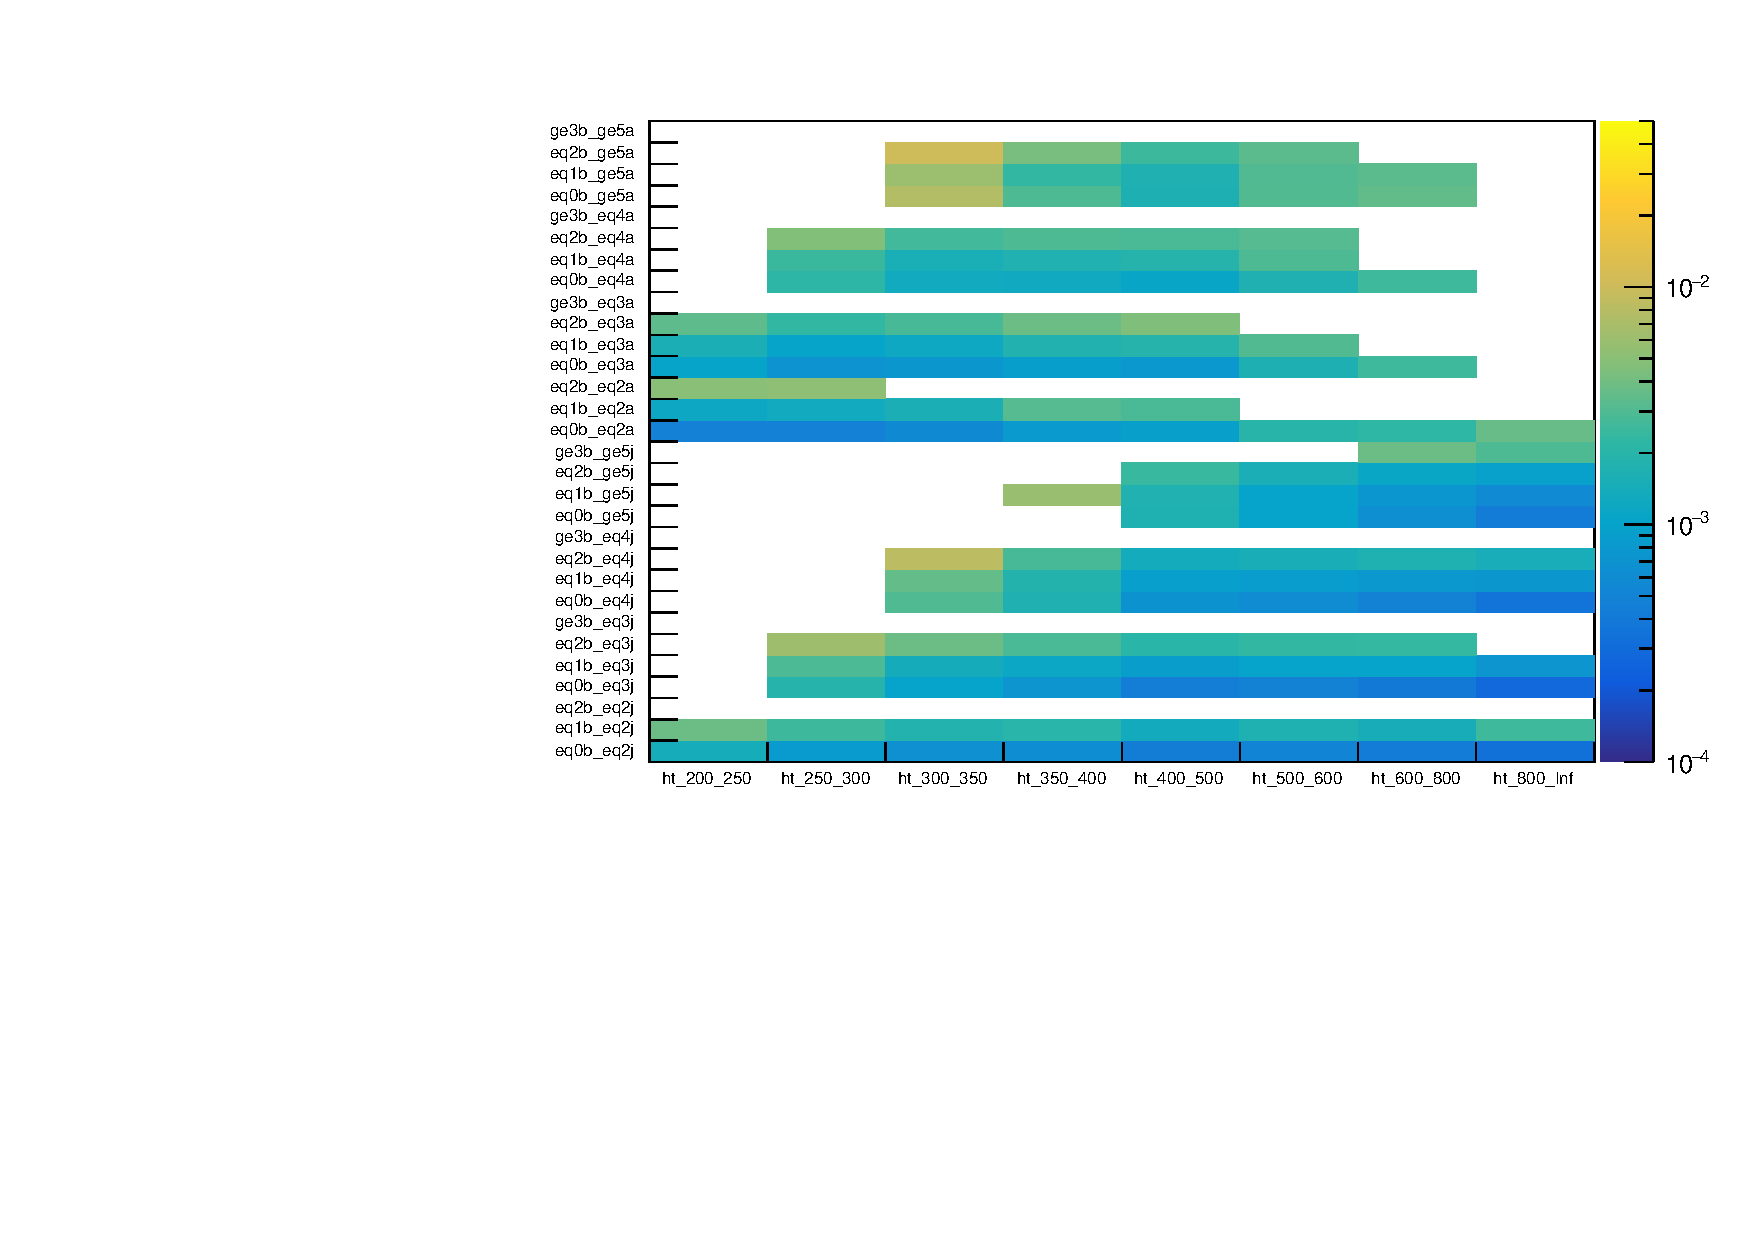
\includegraphics[width=0.5\textwidth]{figures/template13TeV/3fb/frenchFlagErrComplete_Linear2DShiftMean_p1_Zinv.pdf}
%  }\\
%  \caption{\label{fig:expected13} Relative uncertainties per \GeV on the template are shown for \zInv~ in Figure~\ref{fig:zinv13} 
%  and \ttbar/W in Fig.~\ref{fig:ttw13}.}
%  
%\end{figure}%%%

%\begin{figure}[h!]
%  \centering
%  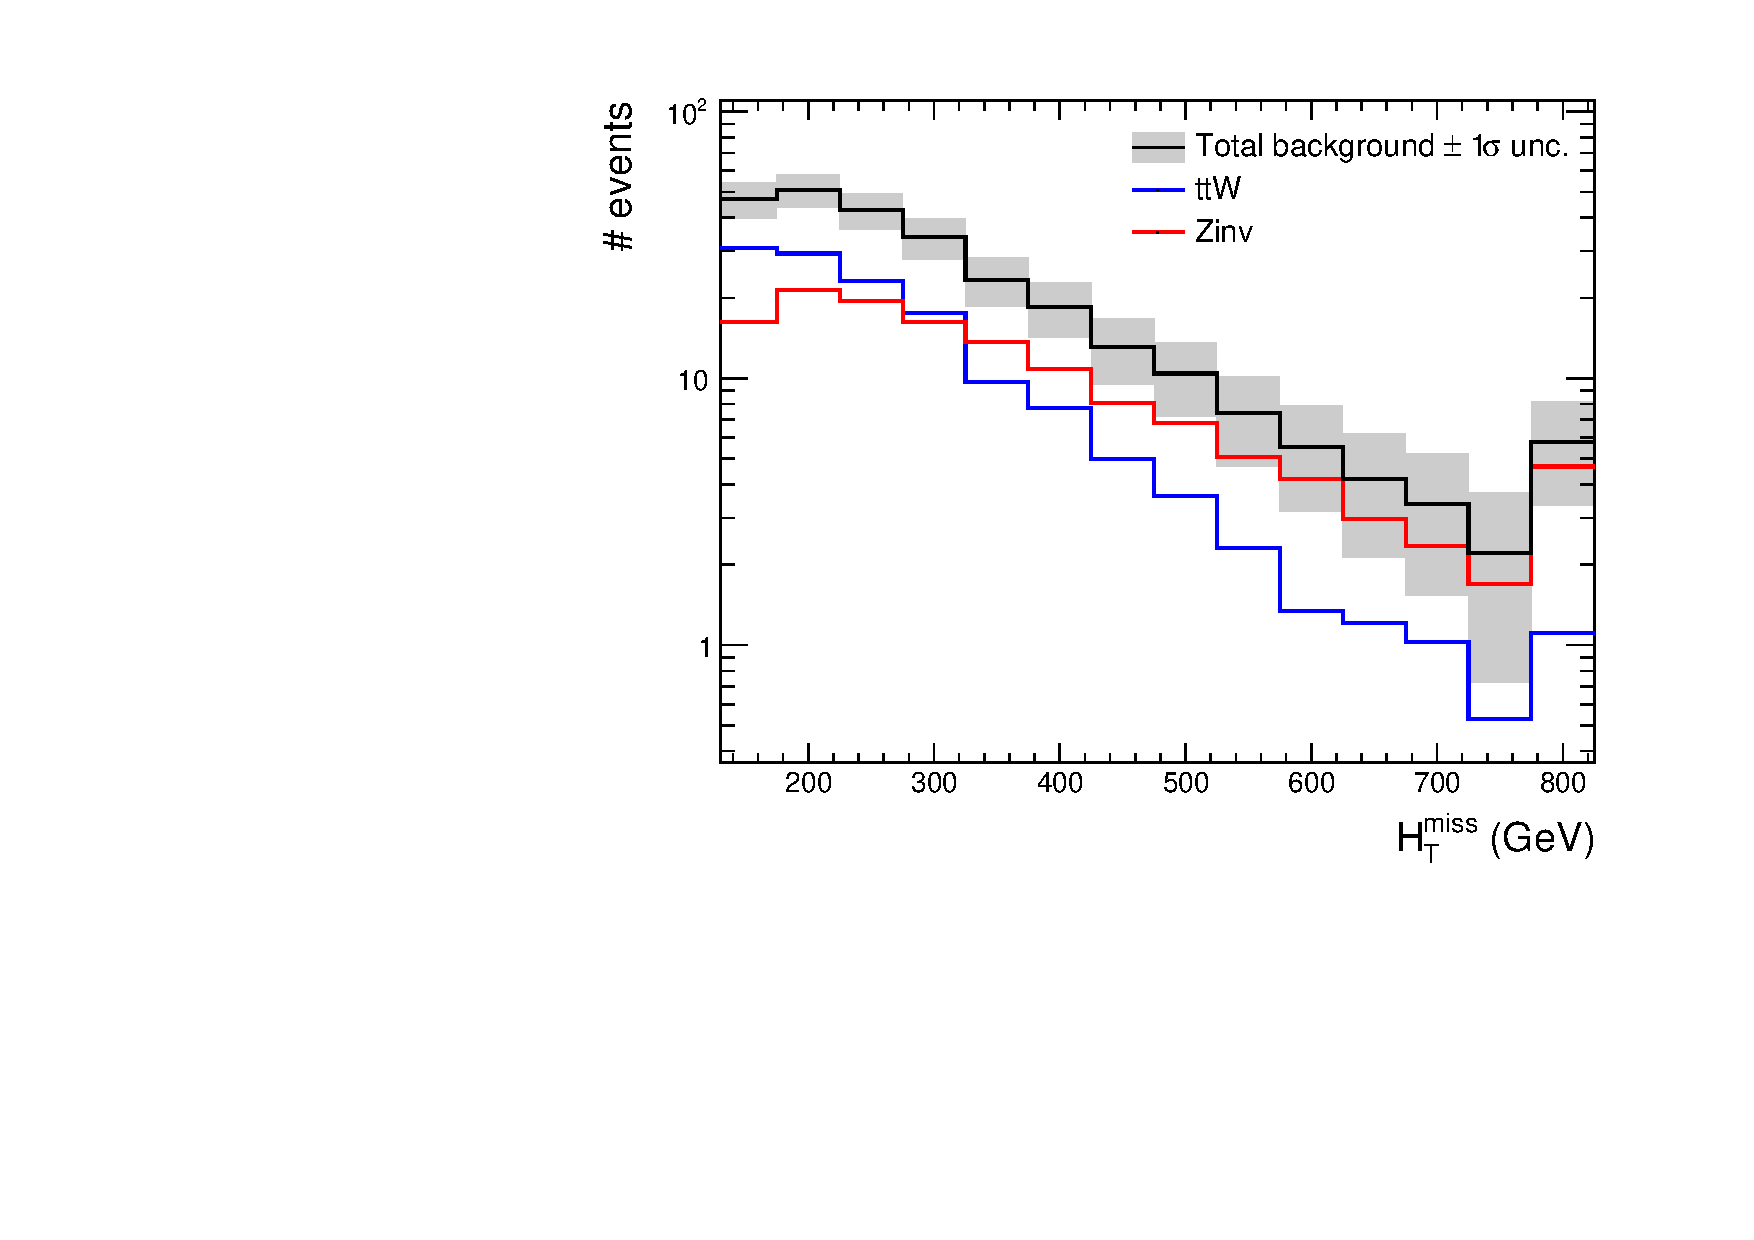
\includegraphics[width=0.5\textwidth]{figures/template/exampleTemplate13TeV.pdf}
%  \\
%  \caption{\label{fig:exampleTemplate13} Example template for 0b,$\ge5$j and $\scalht > 800$\GeV showing the uncertainties from both
%components of the background on the total background prediction.}
  
\end{figure}
